\documentclass{ximera}
\graphicspath{
  {./}
  {1-1QuantitativeReasoning/}
  {1-2RelationsAndGraphs/}
  {1-3ChangingInTandem/}
  {2-1LinearEquations/}
  {2-2LinearModeling/}
  {2-3ExponentialModeling/}
  {3-1WhatIsAFunction/}
  {3-2FunctionProperties/}
  {3-3AverageRatesOfChange/}
  {4-1BuildingNewFunctions/}
  {4-2Polynomials/}
  {5-1RationalFunctions/}
   {5-2ExponentialFunctions/}
  {6-1Domain/}
  {6-2Range/}
  {6-3CompositionOfFunctions/}
  {6-4FunctionTransformations/}
  {7-1ZerosOfFunctions/}
  {7-XZerosOfPolynomials/}
  {7-2ZerosOfFamousFunctions/}
  {8-1SystemsOfEquations/}
  {6-5FunctionTransformationsProject/}
  {1-1QuantitativeReasoning/exercises/}
  {1-2RelationsAndGraphs/exercises/}
  {../1-3ChangingInTandem/exercises/}
  {../2-1LinearEquations/exercises/}
  {../2-2LinearModeling/exercises/}
  {../2-3ExponentialModeling/exercises/}
  {../3-1WhatIsAFunction/exercises/}
  {../3-2FunctionProperties/exercises/}
  {../3-3AverageRatesOfChange/exercises/}
  {../5-2ExponentialFunctions/exercises/}
  {../4-1BuildingNewFunctions/exercises/}
  {../4-2Polynomials/exercises/}
  {../5-1RationalFunctions/exercises/}
  {../6-1Domain/exercises/}
  {../6-2Range/exercises/}
  {../6-3CompositionOfFunctions/exercises/}
  {../7-1ZerosOfFunctions/exercises/}
  {../7-XZerosOfPolynomials/exercises/}
  {../7-2ZerosOfFamousFunctions/exercises/}
  {../6-4FunctionTransformations/exercises/}
  {../8-1SystemsOfEquations/exercises/}
  {../6-3FunctionTransformationsProject/exercises/}
}

\DeclareGraphicsExtensions{.pdf,.png,.jpg,.eps}

\newcommand{\mooculus}{\textsf{\textbf{MOOC}\textnormal{\textsf{ULUS}}}}

\usepackage[makeroom]{cancel} %% for strike outs

\ifxake
\else
\usepackage[most]{tcolorbox}
\fi


%\typeout{************************************************}
%\typeout{New Environments}
%\typeout{************************************************}

%% to fix for web can be removed when deployed offically with ximera2
\let\image\relax\let\endimage\relax
\NewEnviron{image}{% 
  \begin{center}\BODY\end{center}% center
}



\NewEnviron{folder}{
      \addcontentsline{toc}{section}{\textbf{\BODY}}
}

\ifxake
\let\summary\relax
\let\endsummary\relax
\newtheorem*{summary}{Summary}
\newtheorem*{callout}{Callout}
\newtheorem*{overview}{Overview}
\newtheorem*{objectives}{Objectives}
\newtheorem*{motivatingQuestions}{Motivating Questions}
\newtheorem*{MM}{Metacognitive Moment}
      
%% NEEDED FOR XIMERA 2
%\ximerizedEnvironment{summary}
%\ximerizedEnvironment{callout}
%\ximerizedEnvironment{overview} 
%\ximerizedEnvironment{objectives}
%\ximerizedEnvironment{motivatingQuestions}
%\ximerizedEnvironment{MM}
\else
%% CALLOUT
\NewEnviron{callout}{
  \begin{tcolorbox}[colback=blue!5, breakable,pad at break*=1mm]
      \BODY
  \end{tcolorbox}
}
%% MOTIVATING QUESTIONS
\NewEnviron{motivatingQuestions}{
  \begin{tcolorbox}[ breakable,pad at break*=1mm]
    \textbf{\Large Motivating Questions}\hfill
    %\begin{itemize}[label=\textbullet]
      \BODY
    %\end{itemize}
  \end{tcolorbox}
}
%% OBJECTIVES
\NewEnviron{objectives}{  
    \vspace{.5in}
      %\begin{tcolorbox}[colback=orange!5, breakable,pad at break*=1mm]
    \textbf{\Large Learning Objectives}
    \begin{itemize}[label=\textbullet]
      \BODY
    \end{itemize}
    %\end{tcolorbox}
}
%% DEFINITION
\let\definition\relax
\let\enddefinition\relax
\NewEnviron{definition}{
  \begin{tcolorbox}[ breakable,pad at break*=1mm]
    \noindent\textbf{Definition}~
      \BODY
  \end{tcolorbox}
}
%% OVERVIEW
\let\overview\relax
\let\overview\relax
\NewEnviron{overview}{
  \begin{tcolorbox}[ breakable,pad at break*=1mm]
    \textbf{\Large Overview}
    %\begin{itemize}[label=\textbullet] %% breaks Xake
      \BODY
    %\end{itemize}
  \end{tcolorbox}
}
%% SUMMARY
\let\summary\relax
\let\endsummary\relax
\NewEnviron{summary}{
  \begin{tcolorbox}[ breakable,pad at break*=1mm]
    \textbf{\Large Summary}
    %\begin{itemize}[label=\textbullet] %% breaks Xake
      \BODY
    %\end{itemize}
  \end{tcolorbox}
}
%% REMARK
\let\remark\relax
\let\endremark\relax
\NewEnviron{remark}{
  \begin{tcolorbox}[colback=green!5, breakable,pad at break*=1mm]
    \noindent\textbf{Remark}~
      \BODY
  \end{tcolorbox}
}
%% EXPLANATION
\let\explanation\relax
\let\endexplanation\relax
\NewEnviron{explanation}{
    \normalfont
    \noindent\textbf{Explanation}~
      \BODY
}
%% EXPLORATION
\let\exploration\relax
\let\endexploration\relax
\NewEnviron{exploration}{
  \begin{tcolorbox}[colback=yellow!10, breakable,pad at break*=1mm]
    \noindent\textbf{Exploration}~
      \BODY
  \end{tcolorbox}
}
%% METACOGNITIVE MOMENTS
\let\MM\relax
\let\endMM\relax
\NewEnviron{MM}{
  \begin{tcolorbox}[colback=pink!15, breakable,pad at break*=1mm]
    \noindent\textbf{Metacognitive Moment}~
      \BODY
  \end{tcolorbox}
}


\fi





%Notes on what envirnoment to use:  Example with Explanation in text; if they are supposed to answer- Problem; no answer - Exploration


%\typeout{************************************************}
%% Header and footers
%\typeout{************************************************}

\newcommand{\licenseAcknowledgement}{Licensed under Creative Commons 4.0}
\newcommand{\licenseAPC}{\renewcommand{\licenseAcknowledgement}{\textbf{Acknowledgements:} Active Prelude to Calculus (https://activecalculus.org/prelude) }}
\newcommand{\licenseSZ}{\renewcommand{\licenseAcknowledgement}{\textbf{Acknowledgements:} Stitz Zeager Open Source Mathematics (https://www.stitz-zeager.com/) }}
\newcommand{\licenseAPCSZ}{\renewcommand{\licenseAcknowledgement}{\textbf{Acknowledgements:} Active Prelude to Calculus (https://activecalculus.org/prelude) and Stitz Zeager Open Source Mathematics (https://www.stitz-zeager.com/) }}
\newcommand{\licenseORCCA}{\renewcommand{\licenseAcknowledgement}{\textbf{Acknowledgements:}Original source material, products with readable and accessible
math content, and other information freely available at pcc.edu/orcca.}}
\newcommand{\licenseY}{\renewcommand{\licenseAcknowledgement}{\textbf{Acknowledgements:} Yoshiwara Books (https://yoshiwarabooks.org/)}}
\newcommand{\licenseOS}{\renewcommand{\licenseAcknowledgement}{\textbf{Acknowledgements:} OpenStax College Algebra (https://openstax.org/details/books/college-algebra)}}
\newcommand{\licenseAPCSZCSCC}{\renewcommand{\licenseAcknowledgement}{\textbf{Acknowledgements:} Active Prelude to Calculus (https://activecalculus.org/prelude), Stitz Zeager Open Source Mathematics (https://www.stitz-zeager.com/), CSCC PreCalculus and Calculus texts (https://ximera.osu.edu/csccmathematics)}}

\ifxake\else %% do nothing on the website
\usepackage{fancyhdr}
\pagestyle{fancy}
\fancyhf{}
\fancyhead[R]{\sectionmark}
\fancyfoot[L]{\thepage}
\fancyfoot[C]{\licenseAcknowledgement}
\renewcommand{\headrulewidth}{0pt}
\renewcommand{\footrulewidth}{0pt}
\fi

%%%%%%%%%%%%%%%%



%\typeout{************************************************}
%\typeout{Table of Contents}
%\typeout{************************************************}


%% Edit this to change the font style
\newcommand{\sectionHeadStyle}{\sffamily\bfseries}


\makeatletter

%% part uses arabic numerals
\renewcommand*\thepart{\arabic{part}}


\ifxake\else
\renewcommand\chapterstyle{%
  \def\maketitle{%
    \addtocounter{titlenumber}{1}%
    \pagestyle{fancy}
    \phantomsection
    \addcontentsline{toc}{section}{\textbf{\thepart.\thetitlenumber\hspace{1em}\@title}}%
                    {\flushleft\small\sectionHeadStyle\@pretitle\par\vspace{-1.5em}}%
                    {\flushleft\LARGE\sectionHeadStyle\thepart.\thetitlenumber\hspace{1em}\@title \par }%
                    {\setcounter{problem}{0}\setcounter{sectiontitlenumber}{0}}%
                    \par}}





\renewcommand\sectionstyle{%
  \def\maketitle{%
    \addtocounter{sectiontitlenumber}{1}
    \pagestyle{fancy}
    \phantomsection
    \addcontentsline{toc}{subsection}{\thepart.\thetitlenumber.\thesectiontitlenumber\hspace{1em}\@title}%
    {\flushleft\small\sectionHeadStyle\@pretitle\par\vspace{-1.5em}}%
    {\flushleft\Large\sectionHeadStyle\thepart.\thetitlenumber.\thesectiontitlenumber\hspace{1em}\@title \par}%
    %{\setcounter{subsectiontitlenumber}{0}}%
    \par}}



\renewcommand\section{\@startsection{paragraph}{10}{\z@}%
                                     {-3.25ex\@plus -1ex \@minus -.2ex}%
                                     {1.5ex \@plus .2ex}%
                                     {\normalfont\large\sectionHeadStyle}}
\renewcommand\subsection{\@startsection{subparagraph}{10}{\z@}%
                                    {3.25ex \@plus1ex \@minus.2ex}%
                                    {-1em}%
                                    {\normalfont\normalsize\sectionHeadStyle}}

\fi

%% redefine Part
\renewcommand\part{%
   {\setcounter{titlenumber}{0}}
  \if@openright
    \cleardoublepage
  \else
    \clearpage
  \fi
  \thispagestyle{plain}%
  \if@twocolumn
    \onecolumn
    \@tempswatrue
  \else
    \@tempswafalse
  \fi
  \null\vfil
  \secdef\@part\@spart}

\def\@part[#1]#2{%
    \ifnum \c@secnumdepth >-2\relax
      \refstepcounter{part}%
      \addcontentsline{toc}{part}{\thepart\hspace{1em}#1}%
    \else
      \addcontentsline{toc}{part}{#1}%
    \fi
    \markboth{}{}%
    {\centering
     \interlinepenalty \@M
     \normalfont
     \ifnum \c@secnumdepth >-2\relax
       \huge\sffamily\bfseries \partname\nobreakspace\thepart
       \par
       \vskip 20\p@
     \fi
     \Huge \bfseries #2\par}%
    \@endpart}
\def\@spart#1{%
    {\centering
     \interlinepenalty \@M
     \normalfont
     \Huge \bfseries #1\par}%
    \@endpart}
\def\@endpart{\vfil\newpage
              \if@twoside
               \if@openright
                \null
                \thispagestyle{empty}%
                \newpage
               \fi
              \fi
              \if@tempswa
                \twocolumn
                \fi}



\makeatother





%\typeout{************************************************}
%\typeout{Stuff from Ximera}
%\typeout{************************************************}



\usepackage{array}  %% This is for typesetting long division
\setlength{\extrarowheight}{+.1cm}
\newdimen\digitwidth
\settowidth\digitwidth{9}
\def\divrule#1#2{
\noalign{\moveright#1\digitwidth
\vbox{\hrule width#2\digitwidth}}}





\newcommand{\RR}{\mathbb R}
\newcommand{\R}{\mathbb R}
\newcommand{\N}{\mathbb N}
\newcommand{\Z}{\mathbb Z}

\newcommand{\sagemath}{\textsf{SageMath}}


\def\d{\,d}
%\renewcommand{\d}{\mathop{}\!d}
\newcommand{\dd}[2][]{\frac{\d #1}{\d #2}}
\newcommand{\pp}[2][]{\frac{\partial #1}{\partial #2}}
\renewcommand{\l}{\ell}
\newcommand{\ddx}{\frac{d}{\d x}}



%\newcommand{\unit}{\,\mathrm}
\newcommand{\unit}{\mathop{}\!\mathrm}
\newcommand{\eval}[1]{\bigg[ #1 \bigg]}
\newcommand{\seq}[1]{\left( #1 \right)}
\renewcommand{\epsilon}{\varepsilon}
\renewcommand{\phi}{\varphi}


\renewcommand{\iff}{\Leftrightarrow}

\DeclareMathOperator{\arccot}{arccot}
\DeclareMathOperator{\arcsec}{arcsec}
\DeclareMathOperator{\arccsc}{arccsc}
\DeclareMathOperator{\sign}{sign}


%\DeclareMathOperator{\divergence}{divergence}
%\DeclareMathOperator{\curl}[1]{\grad\cross #1}
\newcommand{\lto}{\mathop{\longrightarrow\,}\limits}

\renewcommand{\bar}{\overline}

\colorlet{textColor}{black}
\colorlet{background}{white}
\colorlet{penColor}{blue!50!black} % Color of a curve in a plot
\colorlet{penColor2}{red!50!black}% Color of a curve in a plot
\colorlet{penColor3}{red!50!blue} % Color of a curve in a plot
\colorlet{penColor4}{green!50!black} % Color of a curve in a plot
\colorlet{penColor5}{orange!80!black} % Color of a curve in a plot
\colorlet{penColor6}{yellow!70!black} % Color of a curve in a plot
\colorlet{fill1}{penColor!20} % Color of fill in a plot
\colorlet{fill2}{penColor2!20} % Color of fill in a plot
\colorlet{fillp}{fill1} % Color of positive area
\colorlet{filln}{penColor2!20} % Color of negative area
\colorlet{fill3}{penColor3!20} % Fill
\colorlet{fill4}{penColor4!20} % Fill
\colorlet{fill5}{penColor5!20} % Fill
\colorlet{gridColor}{gray!50} % Color of grid in a plot

\newcommand{\surfaceColor}{violet}
\newcommand{\surfaceColorTwo}{redyellow}
\newcommand{\sliceColor}{greenyellow}




\pgfmathdeclarefunction{gauss}{2}{% gives gaussian
  \pgfmathparse{1/(#2*sqrt(2*pi))*exp(-((x-#1)^2)/(2*#2^2))}%
}





%\typeout{************************************************}
%\typeout{ORCCA Preamble.Tex}
%\typeout{************************************************}


%% \usepackage{geometry}
%% \geometry{letterpaper,total={408pt,9.0in}}
%% Custom Page Layout Adjustments (use latex.geometry)
%% \usepackage{amsmath,amssymb}
%% \usepackage{pgfplots}
\usepackage{pifont}                                         %needed for symbols, s.a. airplane symbol
\usetikzlibrary{positioning,fit,backgrounds}                %needed for nested diagrams
\usetikzlibrary{calc,trees,positioning,arrows,fit,shapes}   %needed for set diagrams
\usetikzlibrary{decorations.text}                           %needed for text following a curve
\usetikzlibrary{arrows,arrows.meta}                         %needed for open/closed intervals
\usetikzlibrary{positioning,3d,shapes.geometric}            %needed for 3d number sets tower

%% NEEDED FOR XIMERA 1
%\usetkzobj{all}       %NO LONGER VALID
%%%%%%%%%%%%%%

\usepackage{tikz-3dplot}
\usepackage{tkz-euclide}                     %needed for triangle diagrams
\usepgfplotslibrary{fillbetween}                            %shade regions of a plot
\usetikzlibrary{shadows}                                    %function diagrams
\usetikzlibrary{positioning}                                %function diagrams
\usetikzlibrary{shapes}                                     %function diagrams
%%% global colors from https://www.pcc.edu/web-services/style-guide/basics/color/ %%%
\definecolor{ruby}{HTML}{9E0C0F}
\definecolor{turquoise}{HTML}{008099}
\definecolor{emerald}{HTML}{1c8464}
\definecolor{amber}{HTML}{c7502a}
\definecolor{amethyst}{HTML}{70485b}
\definecolor{sapphire}{HTML}{263c53}
\colorlet{firstcolor}{sapphire}
\colorlet{secondcolor}{turquoise}
\colorlet{thirdcolor}{emerald}
\colorlet{fourthcolor}{amber}
\colorlet{fifthcolor}{amethyst}
\colorlet{sixthcolor}{ruby}
\colorlet{highlightcolor}{green!50!black}
\colorlet{graphbackground}{white}
\colorlet{wood}{brown!60!white}
%%% curve, dot, and graph custom styles %%%
\pgfplotsset{firstcurve/.style      = {color=firstcolor,  mark=none, line width=1pt, {Kite}-{Kite}, solid}}
\pgfplotsset{secondcurve/.style     = {color=secondcolor, mark=none, line width=1pt, {Kite}-{Kite}, solid}}
\pgfplotsset{thirdcurve/.style      = {color=thirdcolor,  mark=none, line width=1pt, {Kite}-{Kite}, solid}}
\pgfplotsset{fourthcurve/.style     = {color=fourthcolor, mark=none, line width=1pt, {Kite}-{Kite}, solid}}
\pgfplotsset{fifthcurve/.style      = {color=fifthcolor,  mark=none, line width=1pt, {Kite}-{Kite}, solid}}
\pgfplotsset{highlightcurve/.style  = {color=highlightcolor,  mark=none, line width=5pt, -, opacity=0.3}}   % thick, opaque curve for highlighting
\pgfplotsset{asymptote/.style       = {color=gray, mark=none, line width=1pt, <->, dashed}}
\pgfplotsset{symmetryaxis/.style    = {color=gray, mark=none, line width=1pt, <->, dashed}}
\pgfplotsset{guideline/.style       = {color=gray, mark=none, line width=1pt, -}}
\tikzset{guideline/.style           = {color=gray, mark=none, line width=1pt, -}}
\pgfplotsset{altitude/.style        = {dashed, color=gray, thick, mark=none, -}}
\tikzset{altitude/.style            = {dashed, color=gray, thick, mark=none, -}}
\pgfplotsset{radius/.style          = {dashed, thick, mark=none, -}}
\tikzset{radius/.style              = {dashed, thick, mark=none, -}}
\pgfplotsset{rightangle/.style      = {color=gray, mark=none, -}}
\tikzset{rightangle/.style          = {color=gray, mark=none, -}}
\pgfplotsset{closedboundary/.style  = {color=black, mark=none, line width=1pt, {Kite}-{Kite},solid}}
\tikzset{closedboundary/.style      = {color=black, mark=none, line width=1pt, {Kite}-{Kite},solid}}
\pgfplotsset{openboundary/.style    = {color=black, mark=none, line width=1pt, {Kite}-{Kite},dashed}}
\tikzset{openboundary/.style        = {color=black, mark=none, line width=1pt, {Kite}-{Kite},dashed}}
\tikzset{verticallinetest/.style    = {color=gray, mark=none, line width=1pt, <->,dashed}}
\pgfplotsset{soliddot/.style        = {color=firstcolor,  mark=*, only marks}}
\pgfplotsset{hollowdot/.style       = {color=firstcolor,  mark=*, only marks, fill=graphbackground}}
\pgfplotsset{blankgraph/.style      = {xmin=-10, xmax=10,
                                        ymin=-10, ymax=10,
                                        axis line style={-, draw opacity=0 },
                                        axis lines=box,
                                        major tick length=0mm,
                                        xtick={-10,-9,...,10},
                                        ytick={-10,-9,...,10},
                                        grid=major,
                                        grid style={solid,gray!20},
                                        xticklabels={,,},
                                        yticklabels={,,},
                                        minor xtick=,
                                        minor ytick=,
                                        xlabel={},ylabel={},
                                        width=0.75\textwidth,
                                      }
            }
\pgfplotsset{numberline/.style      = {xmin=-10,xmax=10,
                                        minor xtick={-11,-10,...,11},
                                        xtick={-10,-5,...,10},
                                        every tick/.append style={thick},
                                        axis y line=none,
                                        y=15pt,
                                        axis lines=middle,
                                        enlarge x limits,
                                        grid=none,
                                        clip=false,
                                        axis background/.style={},
                                        after end axis/.code={
                                          \path (axis cs:0,0)
                                          node [anchor=north,yshift=-0.075cm] {\footnotesize 0};
                                        },
                                        every axis x label/.style={at={(current axis.right of origin)},anchor=north},
                                      }
            }
\pgfplotsset{openinterval/.style={color=firstcolor,mark=none,ultra thick,{Parenthesis}-{Parenthesis}}}
\pgfplotsset{openclosedinterval/.style={color=firstcolor,mark=none,ultra thick,{Parenthesis}-{Bracket}}}
\pgfplotsset{closedinterval/.style={color=firstcolor,mark=none,ultra thick,{Bracket}-{Bracket}}}
\pgfplotsset{closedopeninterval/.style={color=firstcolor,mark=none,ultra thick,{Bracket}-{Parenthesis}}}
\pgfplotsset{infiniteopeninterval/.style={color=firstcolor,mark=none,ultra thick,{Kite}-{Parenthesis}}}
\pgfplotsset{openinfiniteinterval/.style={color=firstcolor,mark=none,ultra thick,{Parenthesis}-{Kite}}}
\pgfplotsset{infiniteclosedinterval/.style={color=firstcolor,mark=none,ultra thick,{Kite}-{Bracket}}}
\pgfplotsset{closedinfiniteinterval/.style={color=firstcolor,mark=none,ultra thick,{Bracket}-{Kite}}}
\pgfplotsset{infiniteinterval/.style={color=firstcolor,mark=none,ultra thick,{Kite}-{Kite}}}
\pgfplotsset{interval/.style= {ultra thick, -}}
%%% cycle list of plot styles for graphs with multiple plots %%%
\pgfplotscreateplotcyclelist{pccstylelist}{%
  firstcurve\\%
  secondcurve\\%
  thirdcurve\\%
  fourthcurve\\%
  fifthcurve\\%
}
%%% default plot settings %%%
\pgfplotsset{every axis/.append style={
  axis x line=middle,    % put the x axis in the middle
  axis y line=middle,    % put the y axis in the middle
  axis line style={<->}, % arrows on the axis
  scaled ticks=false,
  tick label style={/pgf/number format/fixed},
  xlabel={$x$},          % default put x on x-axis
  ylabel={$y$},          % default put y on y-axis
  xmin = -7,xmax = 7,    % most graphs have this window
  ymin = -7,ymax = 7,    % most graphs have this window
  domain = -7:7,
  xtick = {-6,-4,...,6}, % label these ticks
  ytick = {-6,-4,...,6}, % label these ticks
  yticklabel style={inner sep=0.333ex},
  minor xtick = {-7,-6,...,7}, % include these ticks, some without label
  minor ytick = {-7,-6,...,7}, % include these ticks, some without label
  scale only axis,       % don't consider axis and tick labels for width and height calculation
  cycle list name=pccstylelist,
  tick label style={font=\footnotesize},
  legend cell align=left,
  grid = both,
  grid style = {solid,gray!20},
  axis background/.style={fill=graphbackground},
}}
\pgfplotsset{framed/.style={axis background/.style ={draw=gray}}}
%\pgfplotsset{framed/.style={axis background/.style ={draw=gray,fill=graphbackground,rounded corners=3ex}}}
%%% other tikz (not pgfplots) settings %%%
%\tikzset{axisnode/.style={font=\scriptsize,text=black}}
\tikzset{>=stealth}
%%% for nested diagram in types of numbers section %%%
\newcommand\drawnestedsets[4]{
  \def\position{#1}             % initial position
  \def\nbsets{#2}               % number of sets
  \def\listofnestedsets{#3}     % list of sets
  \def\reversedlistofcolors{#4} % reversed list of colors
  % position and draw labels of sets
  \coordinate (circle-0) at (#1);
  \coordinate (set-0) at (#1);
  \foreach \set [count=\c] in \listofnestedsets {
    \pgfmathtruncatemacro{\cminusone}{\c - 1}
    % label of current set (below previous nested set)
    \node[below=3pt of circle-\cminusone,inner sep=0]
    (set-\c) {\set};
    % current set (fit current label and previous set)
    \node[circle,inner sep=0,fit=(circle-\cminusone)(set-\c)]
    (circle-\c) {};
  }
  % draw and fill sets in reverse order
  \begin{scope}[on background layer]
    \foreach \col[count=\c] in \reversedlistofcolors {
      \pgfmathtruncatemacro{\invc}{\nbsets-\c}
      \pgfmathtruncatemacro{\invcplusone}{\invc+1}
      \node[circle,draw,fill=\col,inner sep=0,
      fit=(circle-\invc)(set-\invcplusone)] {};
    }
  \end{scope}
  }
\ifdefined\tikzset
\tikzset{ampersand replacement = \amp}
\fi
\newcommand{\abs}[1]{\left\lvert#1\right\rvert}
%\newcommand{\point}[2]{\left(#1,#2\right)}
\newcommand{\highlight}[1]{\definecolor{sapphire}{RGB}{59,90,125} {\color{sapphire}{{#1}}}}
\newcommand{\firsthighlight}[1]{\definecolor{sapphire}{RGB}{59,90,125} {\color{sapphire}{{#1}}}}
\newcommand{\secondhighlight}[1]{\definecolor{emerald}{RGB}{20,97,75} {\color{emerald}{{#1}}}}
\newcommand{\unhighlight}[1]{{\color{black}{{#1}}}}
\newcommand{\lowlight}[1]{{\color{lightgray}{#1}}}
\newcommand{\attention}[1]{\mathord{\overset{\downarrow}{#1}}}
\newcommand{\nextoperation}[1]{\mathord{\boxed{#1}}}
\newcommand{\substitute}[1]{{\color{blue}{{#1}}}}
\newcommand{\pinover}[2]{\overset{\overset{\mathrm{\ #2\ }}{|}}{\strut #1 \strut}}
\newcommand{\addright}[1]{{\color{blue}{{{}+#1}}}}
\newcommand{\addleft}[1]{{\color{blue}{{#1+{}}}}}
\newcommand{\subtractright}[1]{{\color{blue}{{{}-#1}}}}
\newcommand{\multiplyright}[2][\cdot]{{\color{blue}{{{}#1#2}}}}
\newcommand{\multiplyleft}[2][\cdot]{{\color{blue}{{#2#1{}}}}}
\newcommand{\divideunder}[2]{\frac{#1}{{\color{blue}{{#2}}}}}
\newcommand{\divideright}[1]{{\color{blue}{{{}\div#1}}}}
\newcommand{\negate}[1]{{\color{blue}{{-}}}\left(#1\right)}
\newcommand{\cancelhighlight}[1]{\definecolor{sapphire}{RGB}{59,90,125}{\color{sapphire}{{\cancel{#1}}}}}
\newcommand{\secondcancelhighlight}[1]{\definecolor{emerald}{RGB}{20,97,75}{\color{emerald}{{\bcancel{#1}}}}}
\newcommand{\thirdcancelhighlight}[1]{\definecolor{amethyst}{HTML}{70485b}{\color{amethyst}{{\xcancel{#1}}}}}
\newcommand{\lt}{<} %% Bart: WHY?
\newcommand{\gt}{>} %% Bart: WHY?
\newcommand{\amp}{&} %% Bart: WHY?


%%% These commands break Xake
%% \newcommand{\apple}{\text{🍎}}
%% \newcommand{\banana}{\text{🍌}}
%% \newcommand{\pear}{\text{🍐}}
%% \newcommand{\cat}{\text{🐱}}
%% \newcommand{\dog}{\text{🐶}}

\newcommand{\apple}{PICTURE OF APPLE}
\newcommand{\banana}{PICTURE OF BANANA}
\newcommand{\pear}{PICTURE OF PEAR}
\newcommand{\cat}{PICTURE OF CAT}
\newcommand{\dog}{PICTURE OF DOG}


%%%%% INDEX STUFF
\newcommand{\dfn}[1]{\textbf{#1}\index{#1}}
\usepackage{imakeidx}
\makeindex[intoc]
\makeatletter
\gdef\ttl@savemark{\sectionmark{}}
\makeatother












 % for drawing cube in Optimization problem
\usetikzlibrary{quotes,arrows.meta}
\tikzset{
  annotated cuboid/.pic={
    \tikzset{%
      every edge quotes/.append style={midway, auto},
      /cuboid/.cd,
      #1
    }
    \draw [every edge/.append style={pic actions, densely dashed, opacity=.5}, pic actions]
    (0,0,0) coordinate (o) -- ++(-\cubescale*\cubex,0,0) coordinate (a) -- ++(0,-\cubescale*\cubey,0) coordinate (b) edge coordinate [pos=1] (g) ++(0,0,-\cubescale*\cubez)  -- ++(\cubescale*\cubex,0,0) coordinate (c) -- cycle
    (o) -- ++(0,0,-\cubescale*\cubez) coordinate (d) -- ++(0,-\cubescale*\cubey,0) coordinate (e) edge (g) -- (c) -- cycle
    (o) -- (a) -- ++(0,0,-\cubescale*\cubez) coordinate (f) edge (g) -- (d) -- cycle;
    \path [every edge/.append style={pic actions, |-|}]
    (b) +(0,-5pt) coordinate (b1) edge ["x"'] (b1 -| c)
    (b) +(-5pt,0) coordinate (b2) edge ["y"] (b2 |- a)
    (c) +(3.5pt,-3.5pt) coordinate (c2) edge ["x"'] ([xshift=3.5pt,yshift=-3.5pt]e)
    ;
  },
  /cuboid/.search also={/tikz},
  /cuboid/.cd,
  width/.store in=\cubex,
  height/.store in=\cubey,
  depth/.store in=\cubez,
  units/.store in=\cubeunits,
  scale/.store in=\cubescale,
  width=10,
  height=10,
  depth=10,
  units=cm,
  scale=.1,
}



\author{David Kish, Debi Stout}
% Source: 1116 Materials



\title{Quantitative Reasoning: Units and Estimates}

\begin{document}
\licenseAPC
\begin{abstract}
We develop our quantitative reasoning skills through units, estimations, and asking `does that make sense'?
\end{abstract}
\maketitle

%\typeout{************************************************}
%\typeout{Rough Estimages}
%\typeout{************************************************}

%\section{Rough Estimates}

%replace color

\section{Units}

Is 12 the same as 1?  As a mathematical value, no 12 and 1 are not the same value.  But if we give these values units, they actually can represent the same thing! \\
What units can we give to 12 and to 1 so that they are equal? 

\begin{center}
12 $\answer{\text{inches}}$ = 1 $\answer{\text{foot}}$
\end{center}


Within our mathematics and science classes, we often think about units in reference to unit conversion. That is, changing from one unit (such as inches) to another unit (such as feet). 

\begin{example} How many inches are in a yard? We might not have this conversion memorized, but if we know the number of inches in a foot and the number of feet in a yard, we can figure it out.

\begin{explanation}
There are 12 inches in every 1 foot. This ratio, written as a fraction, is: 

$$\frac{12 \quad inches}{1 \quad foot}$$

There are 3 feet in every 1 yard. This ratio, written as a fraction, is:
$$  \frac{3 \quad feet}{1 \quad yard} $$

Notice these two fractions have foot/feet in common. Let's use a sketch to help us think about what to do next.

\begin{image}
    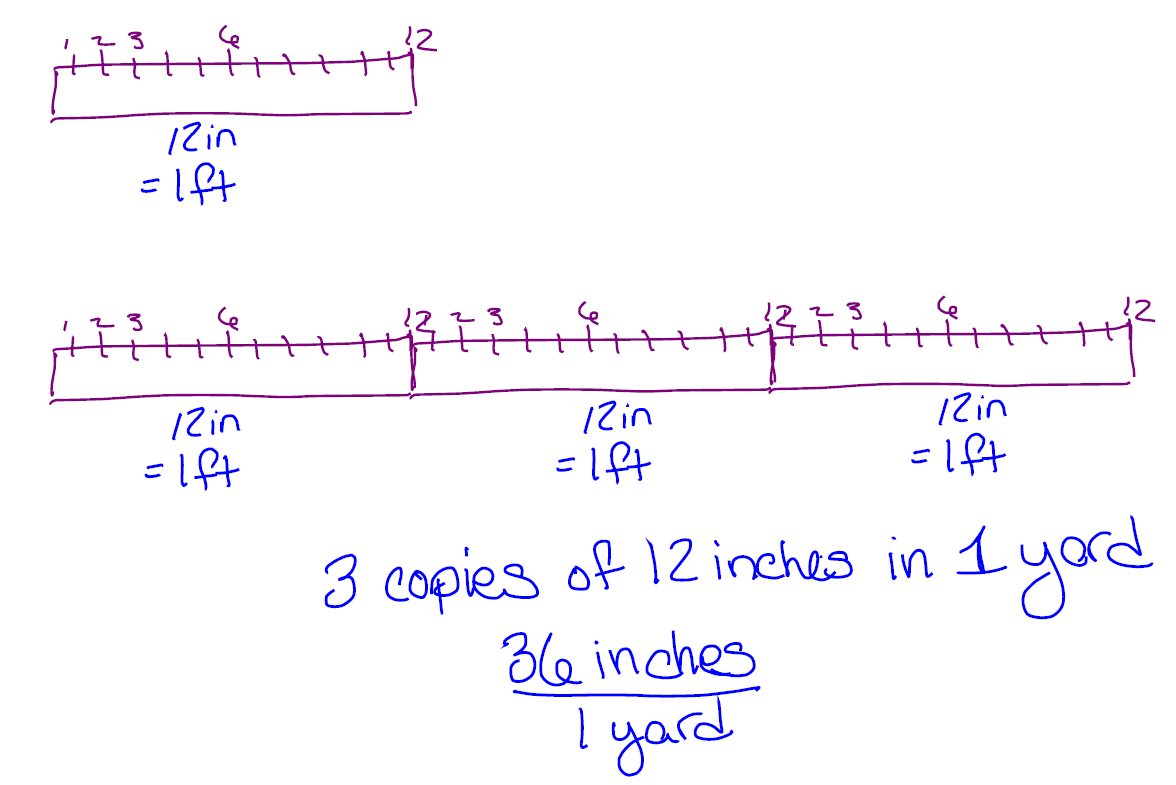
\includegraphics[width=4in]{inchestoyard.png}
\end{image}

We have a $1$ foot ruler comprised of $12$ inches. We know there are $3$ feet in every $1$ yard so we need $3$ copies of that ruler to make $1$ yard. That gives us $3$ rulers of $12$ inches each, $3 \times 12=36$ inches in each $1$ yard.


$$
\frac{12 \quad inches}{1 \quad foot} \times \frac{3 \quad feet}{1 \quad yard} = \frac{12 \quad inches}{1 \quad \cancel{foot}} \times \frac{3 \quad \cancel{feet}}{1 \quad yard} = \frac{36 \quad inches}{1 \quad yard}
$$

\end{explanation}
\end{example}

Let's consider another example. 

\begin{example}

For each of the questions below, determine if the question makes sense.  If it does make sense, find the answer.

\begin{enumerate}[label=\alph*.]
\item How many feet are in a square foot?
\item How many square feet are in a square yard?
\end{enumerate}

\begin{explanation}
Let's look at these questions one at a time.
\begin{enumerate}[label=\alph*.]
\item ``How many feet are in a square foot?''  

This does not make sense.  When we're converting between units, we need to make sure that each of the units is a measurement of the same type.  Feet is a measurement in one dimension (length). Square feet is a measurement in two dimensions (area). Cubic feet is a measurement in three dimensions (volume).  \\

\item ``'How many square feet are in a square yard?''  

Let's draw a picture to help us make sense of this. We'll start by a drawing $1$ foot wide by $1$ foot tall box. This is a square foot. Now, we know that a yard is $3$ feet long so we'll sketch out a $3$ feet wide by $3$ feet tall box. This is our square yard. So our question is, how many square foot boxes fit into our square yard box? 

\begin{image}
    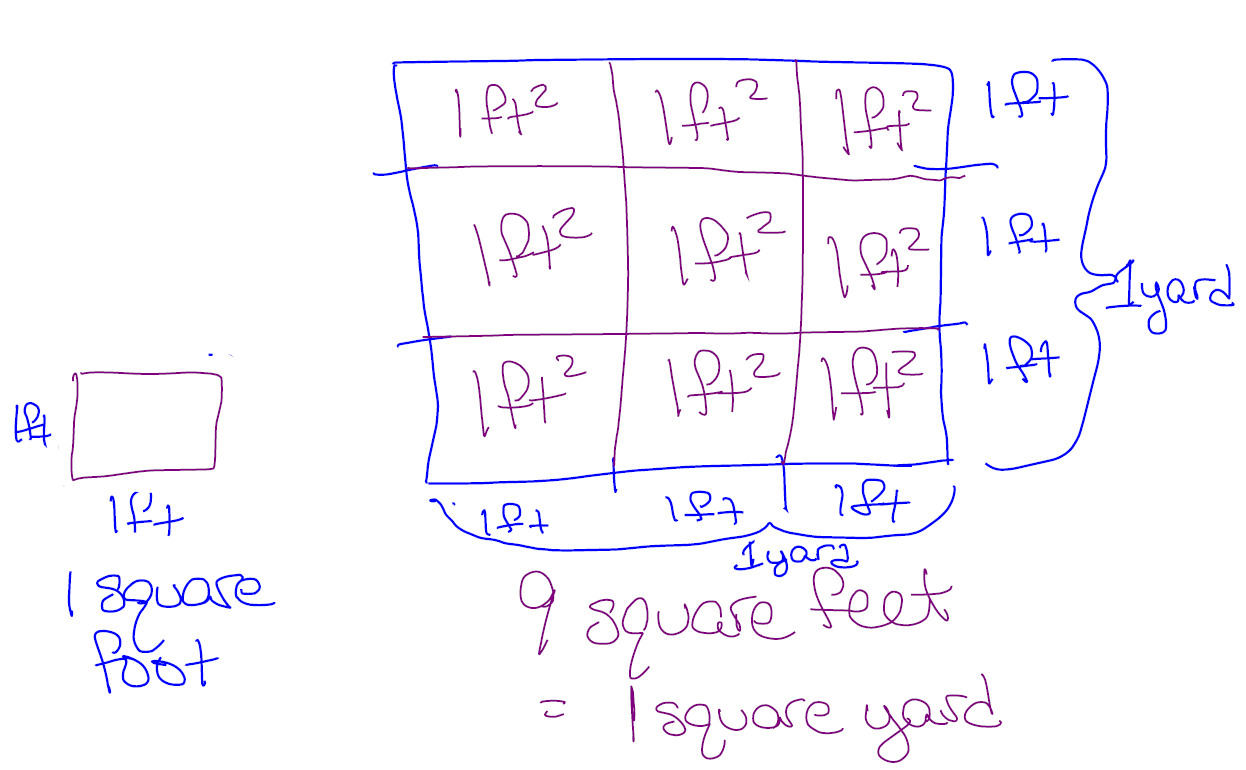
\includegraphics[width=4in]{sqftyd.png}
\end{image}

We see that we have $9$ square foot boxes that fit into the square yard.  There are $9$ square feet in a square yard.\\

\end{enumerate}
\end{explanation}
\end{example}

Now, its time for you try.

\begin{exploration}
Draw a picture to help you solve the following problem: Peyton is helping Alex move into their new apartment. The moving truck is $2$ yards tall, $2$ yards wide, and $3$ yards long. All of the boxes are $1$ cubic foot in volume.  That is, $1$ foot tall, $1$ foot wide, $1$ food long. Assuming the boxes fit perfectly into the truck with no gaps, how many boxes fit into the truck?
\end{exploration}




%\begin{example}
%A typical bottle of wine holds about 24.5 ounces.  How much is this in gallons?\\
%\begin{explanation}
%If we take the original 24.5 ounces in 1 bottle we can set it up as a fraction:

%$$\frac{24.5 \quad ounces}{1 \quad bottle}$$

%There are 128 ounces in 1 gallon. This can be set up as the following fraction:
%$$  \frac{1 \quad gallon}{128 \quad ounces} $$
%These two fractions have ounces in common. We can set the fractions up in such a way that the ounces will ``cancel out.''
%$$
%\frac{24.5 \quad ounces}{1 \quad bottle} \times \frac{1 \quad gallon}{128 \quad ounces} = \frac{24.5 \quad \cancel{ounces}}{1 \quad bottle} \times \frac{1 \quad gallon}{128 \quad \cancel{ounces}} = \frac{0.1914 \quad gallon}{1 \quad bottle}
%$$
%So there are 0.1914 gallons in 1 bottle of wine.
%\end{explanation}
%\end{example}




We use units everyday, even if we don't necessarily think of them as units.  For example, you wouldn't say ``I went to the grocery store and bought $12$.''  $12$ what?  You've given how many you bought (the value), but not how many of what you bought (the units).  Instead you would say ``I went to the grocery store and bought $12$ mangos.'' Units help us communicate mathematics, such as numbers, to others.

What if your friend Arjun told you he had calculated that a board for a dog house needed to be cut $9$? You might scratch your head because $9$ feet seems a bit long for the dog house you're building. Since it doesn't seem to make sense, you ask Arjun to clarify. He says `$9$ inches for the door of the house.' The units not only conveyed information but also helped to answer the question `does that make sense?'

Let's look at another mathematical tool to help us answer the question `does that makes sense?'

\section{Rough Estimates}
Rough estimation allows us to approximate the answer to a question without going through messy calculations. For example, Raquel spends \$$3.68$ on matcha tea per week. How much does Raquel spend on matcha tea per year? Rather than do an exact calculation, we can use an estimate. There are many ways to estimate.  No one way is correct although some are more accurate than others. For example, we can estimate:
$$50 \text{weeks} \times \$4=\$200$$
OR $$50 \text{weeks} \times \$3.5=\$175$$
OR $$55 \text{weeks} \times \$4=\$220$$

Why did we multiply? In our first estimate Raquel spends $\$4$ each time she gets matchta tea and she buys matcha tea $50$ times a year.  So we have $50$ groups of $\$4$.

\begin{image}
    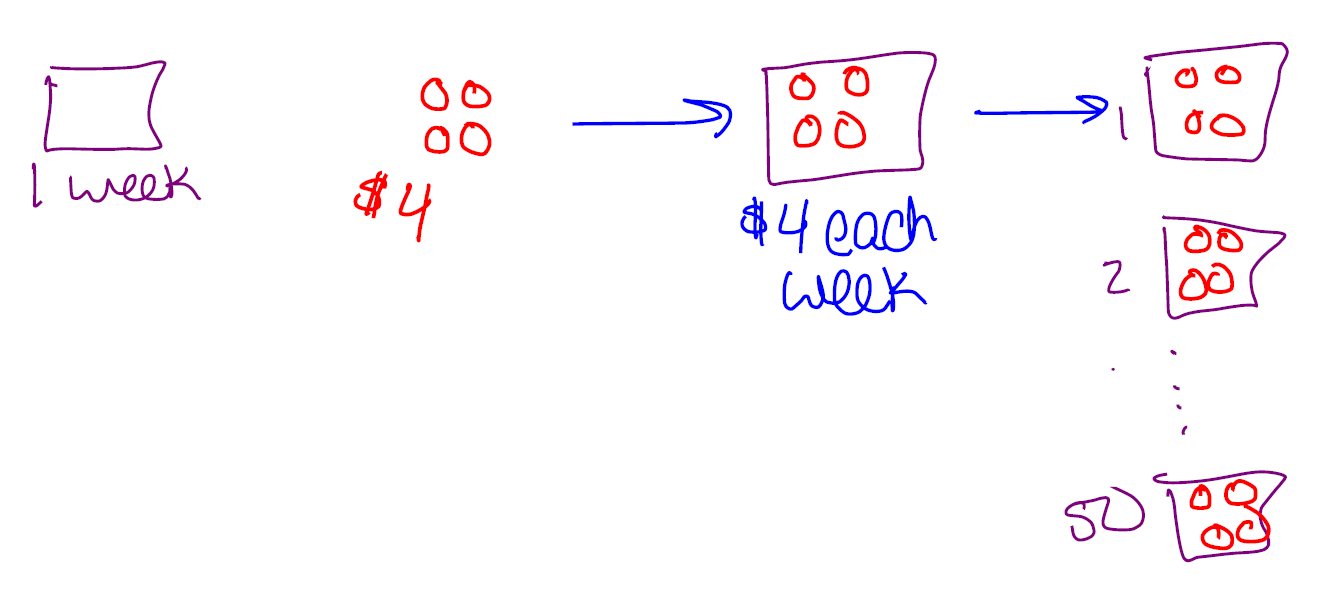
\includegraphics[width=4in]{dollarperyear.png}
\end{image}

What are the units? The \$ may be intuitive but there's another aspect of units here. In our first estimate, Raquel spends $\$200$ on matcha tea \textbf{each year}. `Each year' helps us answer the question, `does that make sense?' $\$200$ of matcha tea each week seems a bit much. $\$200$ of groceries each year seems like too little. Writing answers down in a sentence helps us reason about our units to then be consider if our answer makes sense. Raquel spends $\$200$ on matcha tea each year.

When we estimate, it's often important for us to know whether we have overestimated or underestimated.  Of the above estimates, \$$175$ is an underestimate because we used multiplication and both of the approximate values ($\$3.5$ and $50$ are less than or equal to the actual values.  On the other hand, $\$220$ is an overestimate because $\$4$ and $55$ are greater than or equal to the actual values and multiplying two bigger things results in something bigger. 

\begin{remark}
It is very important to remember that rounding up a number does not always result in an over estimate.  For example, if you divide by a number your rounded up, the resulting answer will actually be smaller!  Always think about what operations you are doing with the numbers when trying to determine if you have an overestimate or underestimate!
\end{remark}

Often the context in which we are estimating will tell us if we prefer to over or under estimate.  If Raquel was trying to determine how much to budget for matcha tea for the year, we would want to overestimate the cost to make sure she has enough money.  However, what if the question was: Matt earns $\$16$ an hour cleaning houses and he work $40$ hours each week. How much money does Matt make per year? Here we want to underestimate the the amount Matt makes so he doesn't run out of money. 

Lets practice by doing an underestimate of how much money Matt makes per year.

\begin{example}
 Matt earns $\$16$ an hour cleaning houses and works $40$ hours each week. Find an underestimate for how much money Matt makes per year.

\begin{explanation}
To underestimate we want to use values that are less than or equal to the given values because we are multiplying. 
\begin{itemize}
\item For $\$16$, depending on how comfortable we are at mental math, we can round down to $\$15$ or use $\$10$. Both are valid. $\$15$ will give us a more accurate estimate but $\$10$ is easier for mental math.  
\item For the hours, we can leave that at $40$ hours since it's already a round number.
\item For $52$ weeks, we can round down to $50$ weeks.
\end{itemize}

We multiply because we have $50$ weeks of $40$ hours of $15$ dollars each hour:
$$50 \text{weeks} \times 40 \text{hours} \times \$15 =\$30000$$
OR $$50 \text{weeks} \times 40 \text{hours} \times \$10 =\$20000$$

Based on our first approximation, Matt earns $\$30000$ each year.
\end{explanation}
\end{example}

\begin{MM}
Note, if we calculated the money Matt makes per year using the exact values, we would find he makes
$$52 \text{weeks} \times 40 \text{hours} \times \$16 =\$33,280$$ 
However, technically this is still an estimate. There are many factors we didn't take into consideration. For example, taxes, benefits, or unpaid sick time that come out of wages.  The number of days in the year doesn't divide evenly into 52 weeks. So some days worked may not be accounted for.  In a later chapter, you'll learn about mathematical models. When we use math to explain situations, we have to made decisions about what information to include.
\end{MM}

Let's try one more example of this type.

\begin{example}
Roughly estimate how many gallons of gasoline Li Wei might use to drive from Columbus, OH to Chicago, IL. The distance to Chicago, IL is about 350 miles (google maps) and Li Wei's car gets about 30 miles per gallon (30 miles = 1 gallon) Explain your answer. Don't forget units!  Also, determine whether your answer is an overestimate or underestimate and which would be preferrable in this situation.

\begin{image}
    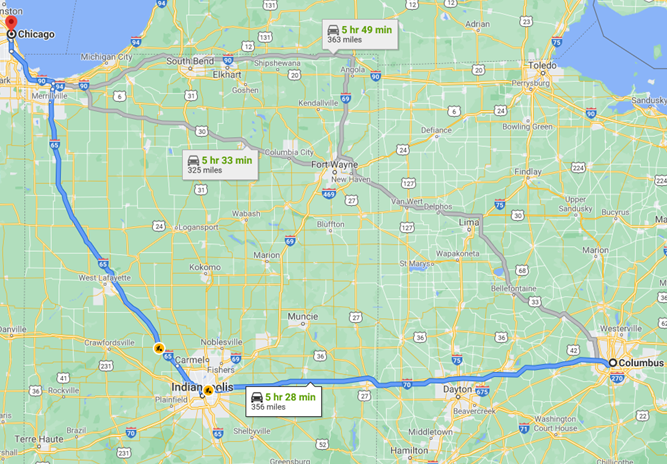
\includegraphics[width=4in]{ColumbusChicago.png}
\end{image}

\begin{explanation}
Li Wei has to drive $350$ miles and for each of those $30$ miles, Li Wei's car will use a gallon of gas.  This question is asking, how many groups of $30$ miles fit into $350$ miles. This is a division problem. 

$$350 \text{mi} \times \frac{1 \text{gal}}{30 \text{mi}}=\frac{350 \text{mi}}{30 \text{mi}} \times{1 \text{gal}}  $$

If we're really good at mental math or have a calculator, we can get an exact number of gallons, but an estimate is good enough. Since we need to divide by $30$, let use a numerator that evenly divides by $30$, such as $360$. So now we have:

$$ \frac{360 \text{mi}}{30\text{mi}} \times{1 \text{gal}}= 12 \text{gallons}$$

Li Wei's car will need approximately 12 gallons of gas for a trip to Chicago, IL.

Now let's consider whether we have made an overestimate or underestimate.  The exact answer would be given by the fraction $\frac{350}{30}$.  Because we increased the numerator of the fraction from $350$ to $360$, we made the entire fraction larger.  Therefore, our estimate is an overestimate.  If we were actually taking a road trip like in this problem, we would want to overestimate the gas we will need so we don't run out of gas!

\end{explanation}
\end{example}

\section{Mathematics doesn't always have one correct answer}

As we've seen with rough estimations, when problem solving, there can be multiple ways to arrive at an answer. Sometimes, we might choose our round numbers based on ease of comptation, but with other problems, we might choose based on personal preferences.  The Pizza Party exploration is an example of this.  There's no one right answer. However, we need to be able to explain our reasoning for our choices and calculations.


\begin{exploration} Pizza Party: 
Work with your group to determine what you would buy for a pizza party in the following scenario.  
You and your roommate are going to have some people over later and so you go to the grocery store to grab some snacks.  Everyone has agreed to pitch in \$10 to pay for pizza and snacks for the night, and you think about 12 people are coming over. Your friends will want an account of how the money was spent so write up an explanation of your reasoning for your choices and calculations.
Here are the prices of various snacks from the grocery store: 
\begin{itemize}
\item Bag of tortilla chips - \$3.99 
\item Salsa - \$3.79
\item Bag of potato chips - \$2.99 
\item Dozen vegan cookies from bakery - \$4.99 
\item Veggie Tray - \$14.99 
\item 12 pack of soda - \$5.79 
\end{itemize}
You want to get at least one of each of these items, but you're also going to order some pizza and breadsticks. 
Here are the prices from your pizza place: 
\begin{itemize}
    \item Cheese flatbread: 
    \begin{itemize}
        \item Medium - \$9.99 
        \item Large - \$11.99 
    \end{itemize}
    \item Cheese cauliflower crust: 
    \begin{itemize}
        \item Medium - \$11.49 
        \item Large - \$13.49 
    \end{itemize}
    \item Breadsticks: 
    \begin{itemize}
        \item 5 for \$4.99 
    \end{itemize}
    \item \$2.49 delivery charge.  Don't forget tip! 
\end{itemize}
You are a good person and do not plan to pocket any of the money that your friends are going to give you to pay for these pizzas and snacks.  Plus, you and your roommate are going to pay for your fairshare (also each pitch in \$10).  Decide what you're going to get and don't forget to write up an explanation of your reasoning for your choices and calculations.
\end{exploration}


%\begin{exploration}
%Roughly estimate how many seconds you've been alive. 
%\begin{itemize}
 %   \item Determine a number that would definitely be way too low for even a rough estimate for each question, but still requires some calculation. Explain why you think this would be unreasonably low. (Still do not use a calculator, use mental arithmetic.) 
  %  \item Determine a number that would definitely be way too high for even a rough estimate for each question. Explain why you think this would be unreasonably high.
  %  \item For each of those problems, do you think your original rough estimation is an underestimate or overestimate? Explain why you think this based off of your calculations. Or if you're not sure if it's under or over, explain why you are unsure.
   % \item If possible, determine a more exact value by using a calculator and not rounding values to get an exact number, or see if google has any estimate(s). Compare this with your original estimations: were you under or over estimating, or can't tell? If you have values to compare, how different are the two values? 
%\end{itemize}
%\end{exploration}





%\begin{exploration}
%\begin{itemize}
%\item``How many ounces are in a yard?'' Explain why this question does not make sense.
%\item``How many feet are in an acre?'' Explain why this question does not make sense.
%\end{itemize}
%Let's talk a little more about this idea highlighted in the question above (about feet and acre units).  It is important to note that feet, square feet, and cubic feet are all different units.  They are not measuring the same thing!  Feet measures length (one dimension), square feet measure area (two dimensions), and cubic feet measure volume (three dimensions).
%\begin{enumerate}
%	\item[Q.] We \textbf{can} convert between \textbf{cubic feet} and {which units} from previous examples?  Why?
%\end{enumerate}
%We can convert between feet and inches, or feet and miles.  Can we convert between square/cubic feet and square/cubic inches, or square/cubic feet and square/cubic miles?  To answer this, we have to ask if these pairs of units are measuring the same property.  If the answer is yes, then yes we can convert between them!
%\begin{itemize}
%\item Do square feet, square inches, and square miles measure the same property?
%\item Do cubic feet, cubic inches, and cubic miles measure the same property?
%\end{itemize}
%In order to convert between units, we need some sort of equivalence.  Just like knowing 4 quarts = 1 gallon, or 16 oz = 1 pound, these are equivalences that we can then use to convert from quarts to gallons or vice versa, or ounces to pounds or vice versa.  
%Let's determine the equivalence for square feet and square inches.
%\begin{image}
%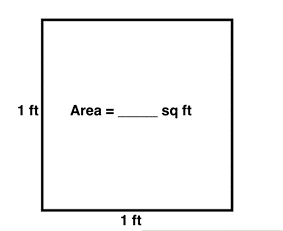
\includegraphics[width=3in]{sqftpic.png} 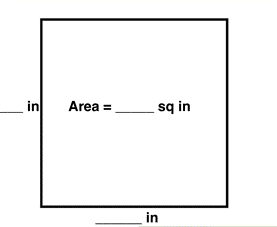
\includegraphics[width=3in]{sqinpic.png}
%\end{image}
%Fill in the blanks above (assume that the squares are the exact same size).
%Since the squares are the exact same size, we can say that $1$ sq ft = $\answer{144}$ sq in.
%Use this same reasoning to determine the equivalence between square miles and square feet:

%$1$ sq mi $= \answer{27878400}$ \quad sq ft

%\end{exploration}


\end{document}
